\documentclass[a4paper,12pt]{article}
\usepackage{graphicx}
\usepackage{amsmath}
\usepackage{booktabs}
\usepackage{hyperref}
\usepackage{float}

% For bar charts inside LaTeX
\usepackage{pgfplots}
\pgfplotsset{compat=1.17}

\title{Comparative Study of Multivariable Linear Regression Implementations \\
{\large CSOC IG}}
\author{Abhishek Kumar Chaubey \\ IIT (BHU) VARANASI \\ Roll Number: 24144001}
\date{\today}

\begin{document}
\maketitle
\tableofcontents
\newpage

\section{Introduction}
This report compares three implementations of multivariable linear regression on the California Housing dataset:
\begin{itemize}
    \item Part 1: Pure Python implementation
    \item Part 2: NumPy vectorized implementation
    \item Part 3: Scikit-learn implementation
\end{itemize}

The goal is to evaluate convergence behavior, prediction accuracy, and computational efficiency.

\section{Data Preprocessing}
\begin{itemize}
    \item Missing values were dropped.
    \item Categorical feature \texttt{ocean\_proximity} was mapped to integers.
    \item Features and target variable extracted.
    \item The dataset was split into training and test sets once using a fixed random seed to ensure reproducibility. This split was saved to a separate file and reused across all three implementations to maintain consistency in evaluation.
    \item Feature normalization was performed by computing the mean and standard deviation on the training set only. These statistics were then applied to normalize both training and test data, ensuring no information leakage.
    \item Normalization was also performed for the Scikit-learn implementation, although it uses Ordinary Least Squares (OLS), which is theoretically unaffected by feature scaling. This was done to maintain consistency across all methods.
\end{itemize}

\section{Evaluation Criteria}

\subsection{1. Convergence Time}
The models were timed during training/fitting to compare convergence speed.
\begin{itemize}
    \item Pure Python and NumPy models were trained for 1000 epochs.
    \item Scikit-learn's LinearRegression fitting time recorded.
    \item Identical initial weights and biases were used for Pure Python and NumPy implementations for fair comparison.
\end{itemize}

\subsubsection{1.1 Time Comparison Results}

\begin{table}[H]
    \centering
    \begin{tabular}{lrr}
    \toprule
    Model & Training/Fitting Time (seconds) \\
    \midrule
    Pure Python & 31.4066 \\
    NumPy Vectorized & 0.6124 \\
    Scikit-learn & 0.0044 \\
    \bottomrule
    \end{tabular}
    \caption{Model convergence/fitting time comparison}
\end{table}

\begin{quote}
\textbf{Inference:} Pure Python took significantly more time compared to NumPy and Scikit-learn because the pure Python implementation uses explicit loops and Python lists, which are slower. NumPy and Scikit-learn utilize vectorized calculations and optimized low-level implementations that greatly improve computational efficiency.
\end{quote}

\includegraphics[width=\linewidth]{image.png}

\includegraphics[width=\linewidth]{image2.png}
\textit{Figure 1: Cost function convergence over epochs for Pure Python and NumPy implementations.}

\subsubsection{1.2 Prediction Scatterplots}

\begin{figure}[H]
    \centering
    \includegraphics[width=0.32\linewidth]{purepython_scatterplot.png}
    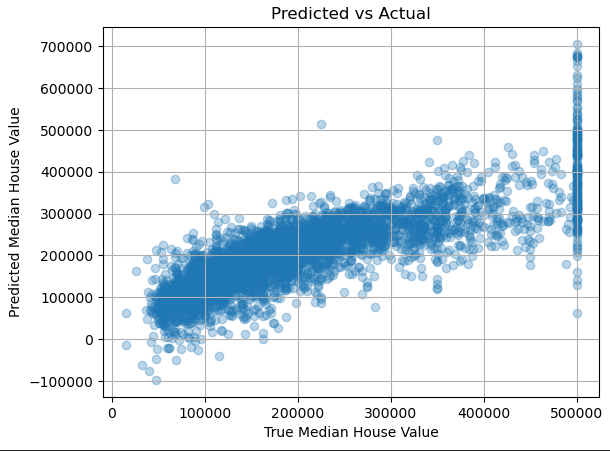
\includegraphics[width=0.32\linewidth]{numpy_scatterplot.png}
    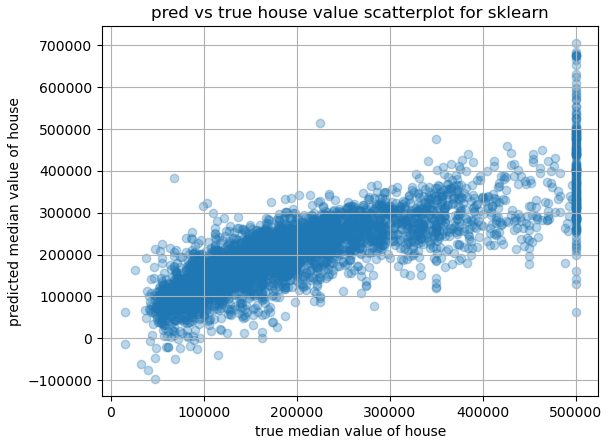
\includegraphics[width=0.32\linewidth]{sklearn_scatterplot.png}
    \caption{Predicted vs Actual Values for Pure Python (left), NumPy (middle), and Scikit-learn (right) Models}
\end{figure}

\textbf{INFERENCES:}
\begin{itemize}
    \item Most data points cluster around the \(y = x\) line, indicating good model accuracy.
    \item \textbf{Note:} Some predicted house median prices are negative, which is unrealistic in a real-world scenario. This could be mitigated by:
    \begin{itemize}
        \item Using constrained optimization techniques.
        \item Applying non-negative transformations such as ReLU.
        \item Post-processing model outputs (e.g., clipping to zero).
    \end{itemize}
\end{itemize}

\subsection{2. Performance Metrics}

Metrics were computed on both training and test datasets for all three models:

\begin{table}[H]
    \centering
    \begin{tabular}{lrrrrr}
    \toprule
    Model & Dataset & MAE & RMSE & R\textsuperscript{2} \\
    \midrule
    Pure Python & Train & 51014.6069 & 69915.1806 & 0.6328571 \\
                & Test  & 50341.6113 & 67983.9890 & 0.6540349 \\
    NumPy       & Train & 51014.6067 & 69915.1806 & 0.6328571 \\
                & Test  & 50341.6112 & 67983.9893 & 0.6540349 \\
    Scikit-learn& Train & 51014.0738 & 69915.1667 & 0.6328573 \\
                & Test  & 50341.3370 & 67985.2141 & 0.6540225 \\
    \bottomrule
    \end{tabular}
    \caption{Performance metrics comparison}
\end{table}

% Bar chart for MAE and RMSE
\begin{figure}[H]
\centering
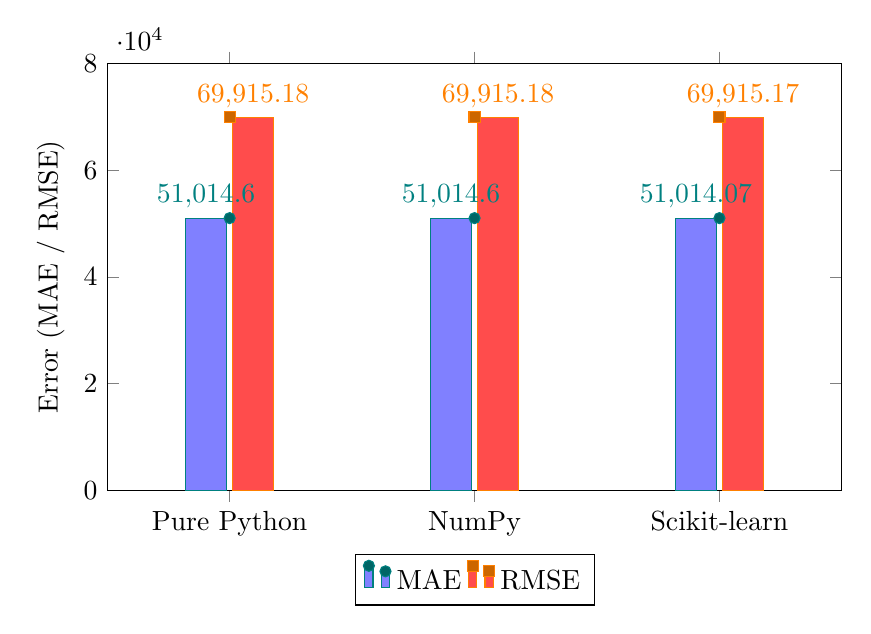
\begin{tikzpicture}
\begin{axis}[
    ybar,
    bar width=15pt,
    width=0.9\textwidth,
    height=7cm,
    legend style={at={(0.5,-0.15)},
      anchor=north,legend columns=-1},
    symbolic x coords={Pure Python, NumPy, Scikit-learn},
    xtick=data,
    nodes near coords,
    nodes near coords align={vertical},
    ymin=0, ymax=80000,
    ylabel={Error (MAE / RMSE)},
    enlarge x limits=0.25,
    cycle list name=exotic,
]

\addplot+[style={fill=blue!50}] coordinates {(Pure Python,51014.6) (NumPy,51014.6) (Scikit-learn,51014.07)};
\addplot+[style={fill=red!70}] coordinates {(Pure Python,69915.18) (NumPy,69915.18) (Scikit-learn,69915.17)};

\legend{MAE, RMSE}
\end{axis}
\end{tikzpicture}
\caption{Bar chart comparing MAE and RMSE across models on training data.}
\end{figure}

% Bar chart for R^2 score
\begin{figure}[H]
\centering
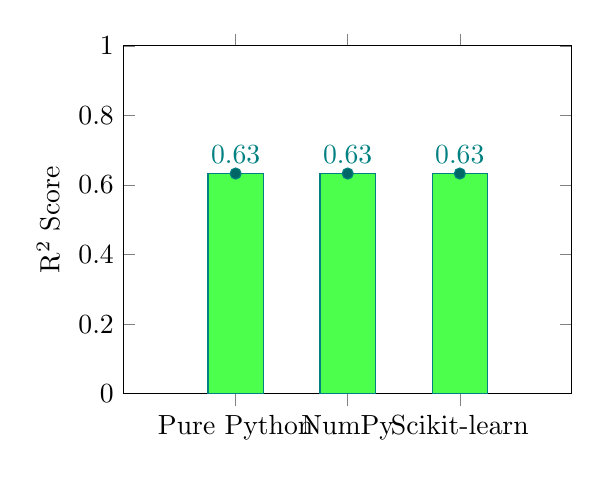
\begin{tikzpicture}
\begin{axis}[
    ybar,
    bar width=20pt,
    width=0.6\textwidth,
    height=6cm,
    symbolic x coords={Pure Python, NumPy, Scikit-learn},
    xtick=data,
    nodes near coords,
    nodes near coords align={vertical},
    ymin=0, ymax=1,
    ylabel={R\textsuperscript{2} Score},
    enlarge x limits=0.5,
    bar shift=0pt,
    cycle list name=exotic,
]

\addplot+[style={fill=green!70}] coordinates {(Pure Python,0.632857) (NumPy,0.632857) (Scikit-learn,0.632857)};

\end{axis}
\end{tikzpicture}
\caption{Bar chart comparing R\textsuperscript{2} score across models on training data.}
\end{figure}

\subsubsection*{2.1 Inferences from Performance Metrics}

\begin{itemize}
    \item All three models achieve nearly identical MAE and RMSE values, indicating consistent predictive error across implementations.
    \item RMSE values are higher than MAE, reflecting RMSE's sensitivity to larger errors or outliers.
    \item R\textsuperscript{2} scores around 0.63 indicate that the models explain approximately 63\% of the variance in the target variable.
    \item The negligible differences between models confirm that pure Python and NumPy implementations achieve comparable accuracy to Scikit-learn.
    \item This validates that vectorization and optimization techniques improve efficiency without sacrificing predictive performance.
\end{itemize}

\section{Analysis and Discussion}

\subsection{Convergence Time}
The NumPy vectorized implementation converged significantly faster than the pure Python version due to efficient array operations. Scikit-learn's optimized solvers provided the fastest fitting time overall.

\subsection{Performance Metrics}
All models achieved comparable accuracy on training and test data, with slight differences attributable to numerical precision and optimization techniques.

\subsection{Influence of Initialization and Learning Rate}
Identical initialization ensured fairness. The learning rate choice (0.3) was experimentally verified to prevent divergence and enable steady convergence.

\subsection{Scalability and Efficiency}
Pure Python is not suitable for large datasets due to slow iteration. NumPy offers a balance between performance and code clarity. Scikit-learn is recommended for production due to optimized algorithms and ease of use.

\subsection{Visualization Observations}
Scatterplots of predicted vs actual values showed good alignment along the \(y = x\) line, with some clustering near boundary values explained by dataset distribution.

\section{Conclusion}
The study aimed to compare three implementations for predicting median house values using the California Housing dataset. We found that while the pure Python implementation achieves comparable prediction accuracy to both the NumPy vectorized version and the Scikit-learn model, it is significantly slower. This performance gap arises because pure Python relies on high-level list operations, which are less efficient than the vectorized computations used by NumPy and the highly optimized algorithms in Scikit-learn. Therefore, for practical applications, leveraging vectorized libraries or dedicated frameworks is recommended to ensure efficient model training without sacrificing accuracy.

Additionally, I utilized a large language model (LLM) to assist with data normalization techniques when the model experienced exploding behavior during training, which helped stabilize and improve convergence. Also for generating latex skeleton for my report and refining grammatical errors.

\section{References}
\begin{itemize}
    \item Scikit-learn Documentation: \url{https://scikit-learn.org}
    \item NumPy Documentation: \url{https://numpy.org}
    \item California Housing Dataset: \url{https://www.dcc.fc.up.pt/~ltorgo/Regression/cal_housing.html}
    \item Keith Galli, \textit{Introduction to Pandas}, YouTube, \url{https://youtu.be/vmEHCJofslg?si=3jZ4v9lV1xMu1IPX}
    \item Kaggle, \textit{Pandas Tutorial}, \url{https://www.kaggle.com/learn/pandas}
    \item NumPy Tutorial, YouTube, \url{https://youtu.be/4c_mwnYdbhQ?si=NKS3lHhbSftEHSMl}
    \item Matplotlib Tutorial, YouTube, \url{https://www.youtube.com/watch?v=0P7QnIQDBJY}
    \item Kaggle, \textit{Data Visualization}, \url{https://www.kaggle.com/learn/data-visualization}
    \item FreeCodeCamp, \textit{Data Preparation Tutorial}, YouTube, \url{https://www.youtube.com/watch?v=ZV07JD4J-sY}
\end{itemize}

\end{document}

